% !TEX program = pdflatex
\documentclass{article}
% FONTS
\usepackage[T1]{fontenc}
\usepackage{tgtermes}
\usepackage{amsmath}

% GEOMETRY
\usepackage[
  paper  = letterpaper,
  left   = 1.65in,
  right  = 1.65in,
  top    = 0.5in,
  bottom = 1.0in,
  ]{geometry}

% COLOR
\usepackage[usenames,dvipsnames]{xcolor}
\definecolor{shadecolor}{gray}{0.9}

% SPACING and TEXT
\usepackage[final,expansion=alltext]{microtype}
\usepackage[english]{babel}
\usepackage[parfill]{parskip}
\usepackage{afterpage}
\usepackage{framed}
\usepackage{nicefrac}
\pagenumbering{gobble}

% COUNTERS
\renewcommand{\labelenumi}{\color{black!67}{\arabic{enumi}.}}
\renewcommand{\labelenumii}{{\color{black!67}(\alph{enumii})}}
\renewcommand{\labelitemi}{{\color{black!67}\textbullet}}

% FIGURES
\usepackage{graphicx}
\usepackage[labelfont=bf]{caption}
\usepackage[format=hang]{subcaption}

% TABLES
\usepackage{booktabs}

% BIBLIOGRAPHY
\usepackage{natbib}

% ALGORITHMS
\usepackage[algoruled]{algorithm2e}
\usepackage{listings}
\usepackage{fancyvrb}
\fvset{fontsize=\normalsize}

% HYPERREF
\usepackage[colorlinks,linktoc=all]{hyperref}
\usepackage[all]{hypcap}
\hypersetup{citecolor=Violet}
\hypersetup{linkcolor=black}
\hypersetup{urlcolor=MidnightBlue}

% CLEVEREF must come after HYPERREF
\usepackage[nameinlink]{cleveref}

% COLOR DEFINITIONS
\newcommand{\red}[1]{\textcolor{BrickRed}{#1}}
\newcommand{\orange}[1]{\textcolor{BurntOrange}{#1}}
\newcommand{\green}[1]{\textcolor{OliveGreen}{#1}}
\newcommand{\blue}[1]{\textcolor{MidnightBlue}{#1}}
\newcommand{\gray}[1]{\textcolor{black!60}{#1}}

% LISTINGS
\usepackage{listings}


% !TEX root = template.tex

% \DeclareRobustCommand{\mb}[1]{\ensuremath{\boldsymbol{\mathbf{#1}}}}
\DeclareRobustCommand{\mb}[1]{\mathbold{#1}}

% \newcommand{\KL}[2]{\ensuremath{\textrm{KL}\PARENS{#1\;\|\;#2}}}
\DeclareRobustCommand{\KL}[2]{\ensuremath{\textrm{KL}\left(#1\;\|\;#2\right)}}

\DeclareMathOperator*{\argmax}{arg\,max}
\DeclareMathOperator*{\argmin}{arg\,min}

\renewcommand{\mid}{~\vert~}
\newcommand{\g}{\mid}
\newcommand{\prm}{~;~}

\newcommand{\mba}{\mb{a}}
\newcommand{\mbb}{\mb{b}}
\newcommand{\mbc}{\mb{c}}
\newcommand{\mbd}{\mb{d}}
\newcommand{\mbe}{\mb{e}}
\newcommand{\mbg}{\mb{g}}
\newcommand{\mbh}{\mb{h}}
\newcommand{\mbi}{\mb{i}}
\newcommand{\mbj}{\mb{j}}
\newcommand{\mbk}{\mb{k}}
\newcommand{\mbl}{\mb{l}}
\newcommand{\mbm}{\mb{m}}
\newcommand{\mbn}{\mb{n}}
\newcommand{\mbo}{\mb{o}}
\newcommand{\mbp}{\mb{p}}
\newcommand{\mbq}{\mb{q}}
\newcommand{\mbr}{\mb{r}}
\newcommand{\mbs}{\mb{s}}
\newcommand{\mbt}{\mb{t}}
\newcommand{\mbu}{\mb{u}}
\newcommand{\mbv}{\mb{v}}
\newcommand{\mbw}{\mb{w}}
\newcommand{\mbx}{\mb{x}}
\newcommand{\mby}{\mb{y}}
\newcommand{\mbz}{\mb{z}}

\newcommand{\mbA}{\mb{A}}
\newcommand{\mbB}{\mb{B}}
\newcommand{\mbC}{\mb{C}}
\newcommand{\mbD}{\mb{D}}
\newcommand{\mbE}{\mb{E}}
\newcommand{\mbF}{\mb{F}}
\newcommand{\mbG}{\mb{G}}
\newcommand{\mbH}{\mb{H}}
\newcommand{\mbI}{\mb{I}}
\newcommand{\mbJ}{\mb{J}}
\newcommand{\mbK}{\mb{K}}
\newcommand{\mbL}{\mb{L}}
\newcommand{\mbM}{\mb{M}}
\newcommand{\mbN}{\mb{N}}
\newcommand{\mbO}{\mb{O}}
\newcommand{\mbP}{\mb{P}}
\newcommand{\mbQ}{\mb{Q}}
\newcommand{\mbR}{\mb{R}}
\newcommand{\mbS}{\mb{S}}
\newcommand{\mbT}{\mb{T}}
\newcommand{\mbU}{\mb{U}}
\newcommand{\mbV}{\mb{V}}
\newcommand{\mbW}{\mb{W}}
\newcommand{\mbX}{\mb{X}}
\newcommand{\mbY}{\mb{Y}}
\newcommand{\mbZ}{\mb{Z}}

\newcommand{\mbalpha}{\mb{\alpha}}
\newcommand{\mbbeta}{\mb{\beta}}
\newcommand{\mbdelta}{\mb{\delta}}
\newcommand{\mbepsilon}{\mb{\epsilon}}
\newcommand{\mbchi}{\mb{\chi}}
\newcommand{\mbeta}{\mb{\eta}}
\newcommand{\mbgamma}{\mb{\gamma}}
\newcommand{\mbiota}{\mb{\iota}}
\newcommand{\mbkappa}{\mb{\kappa}}
\newcommand{\mblambda}{\mb{\lambda}}
\newcommand{\mbmu}{\mb{\mu}}
\newcommand{\mbnu}{\mb{\nu}}
\newcommand{\mbomega}{\mb{\omega}}
\newcommand{\mbphi}{\mb{\phi}}
\newcommand{\mbpi}{\mb{\pi}}
\newcommand{\mbpsi}{\mb{\psi}}
\newcommand{\mbrho}{\mb{\rho}}
\newcommand{\mbsigma}{\mb{\sigma}}
\newcommand{\mbtau}{\mb{\tau}}
\newcommand{\mbtheta}{\mb{\theta}}
\newcommand{\mbupsilon}{\mb{\upsilon}}
\newcommand{\mbvarepsilon}{\mb{\varepsilon}}
\newcommand{\mbvarphi}{\mb{\varphi}}
\newcommand{\mbvartheta}{\mb{\vartheta}}
\newcommand{\mbvarrho}{\mb{\varrho}}
\newcommand{\mbxi}{\mb{\xi}}
\newcommand{\mbzeta}{\mb{\zeta}}

\newcommand{\mbDelta}{\mb{\Delta}}
\newcommand{\mbGamma}{\mb{\Gamma}}
\newcommand{\mbLambda}{\mb{\Lambda}}
\newcommand{\mbOmega}{\mb{\Omega}}
\newcommand{\mbPhi}{\mb{\Phi}}
\newcommand{\mbPi}{\mb{\Pi}}
\newcommand{\mbPsi}{\mb{\Psi}}
\newcommand{\mbSigma}{\mb{\Sigma}}
\newcommand{\mbTheta}{\mb{\Theta}}
\newcommand{\mbUpsilon}{\mb{\Upsilon}}
\newcommand{\mbXi}{\mb{\Xi}}

\newcommand{\mbone}{\mbf{1}}
\newcommand{\mbzero}{\mbf{0}}


\newcommand{\dif}{\mathop{}\!\mathrm{d}}
\newcommand{\diag}{\textrm{diag}}
\newcommand{\supp}{\textrm{supp}}

\newcommand{\E}{\mathbb{E}}
\newcommand{\Var}{\mathbb{V}\textrm{ar}}
\newcommand{\bbH}{\mathbb{H}}

\newcommand{\bbN}{\mathbb{N}}
\newcommand{\bbZ}{\mathbb{Z}}
\newcommand{\bbR}{\mathbb{R}}
\newcommand{\bbS}{\mathbb{S}}

\newcommand{\cA}{\mathcal{A}}
\newcommand{\cB}{\mathcal{B}}
\newcommand{\cC}{\mathcal{C}}
\newcommand{\cD}{\mathcal{D}}
\newcommand{\cE}{\mathcal{E}}
\newcommand{\cF}{\mathcal{F}}
\newcommand{\cG}{\mathcal{G}}
\newcommand{\cH}{\mathcal{H}}
\newcommand{\cI}{\mathcal{I}}
\newcommand{\cJ}{\mathcal{J}}
\newcommand{\cK}{\mathcal{K}}
\newcommand{\cL}{\mathcal{L}}
\newcommand{\cM}{\mathcal{M}}
\newcommand{\cN}{\mathcal{N}}
\newcommand{\cO}{\mathcal{O}}
\newcommand{\cP}{\mathcal{P}}
\newcommand{\cQ}{\mathcal{Q}}
\newcommand{\cR}{\mathcal{R}}
\newcommand{\cS}{\mathcal{S}}
\newcommand{\cT}{\mathcal{T}}
\newcommand{\cU}{\mathcal{U}}
\newcommand{\cV}{\mathcal{V}}
\newcommand{\cW}{\mathcal{W}}
\newcommand{\cX}{\mathcal{X}}
\newcommand{\cY}{\mathcal{Y}}
\newcommand{\cZ}{\mathcal{Z}}

\newcommand{\Gam}{\textrm{Gam}}
\newcommand{\InvGam}{\textrm{InvGam}}


\begin{document}

\title{\textbf{Forecasting Counties in Danger of Drought in California Using Prophet}}
\date{\today}
\author{Vikram Rajan - vjr2123}

\maketitle

\begin{abstract}
    My project revolves around the early detection of states that potentially could be entering or nearing a drought or dry-phase, and seeing if there are nearby states or counties within a particular state that themselves are not in danger and thus could provide aid. Droughts are one of the worst things to happen to a state, as in addition to creating shortages of drinking water, they lead to a myriad of other problems including air quality, sanitation and hygiene, food and nutrition, and the overall economy of a state. Using an open-source forecasting tool called Prophet, released by Facebook, I created a model that takes in historical monthly precipitation from all counties in California and determines the risk it is in of drought. The results were validated against data from the US Drought Monitor's own drought predictor, and it performed very well. The model creates a dictionary which is then fed into a choropleth-map generator to conveniently display the results. 

\end{abstract}


\section{Introduction}
Droughts are defined as a prolonged period of abnormally low rainfall. On top of creating shortages of drinking water, they lead to a myriad of other environmental issues, such as impacts on air quality, sanitation and hygiene, food and nutrition, and the economy. A 2020 study published by Science found climate change responsible for an increase in "anthropogenic trends in temperature, relative humidity, and precipitation" and  these trends account for "46\% of the 2000–2018 drought severity \cite{Science}." This correlation between climate change and drought frequency and intensity has created an urgency amongst machine learning scientists for drought predicting models in an attempt to mitigate these impacts. 

California has been one of the states most impacted by droughts, as the past two decades the state has been abnormally dry and warm, and also experienced the worst drought in its recorded history. In addition to the water shortages and detrimental affect on agriculture, these conditions have resulted in damaged forests, intensified wildfires, worse hydroelectricity generation, and depleted groundwater aquifers. On top of all this, severe drought just last year caused the loss of an estimated 8500 jobs in the California agriculture industry, as well as \$1.2 billion dollars in direct costs. For these reasons, this model focuses on the 58 counties of California, attempting to create a model that can accurately assess a county's level of danger for being in a drought. The model will analyze historical precipitation data for each county and forecast values using an open-source tool called Prophet, which when will then be compared to the actual rainfall amounts. The result will be an easily interpretable choropleth map, allowing one to quickly and visually determine what local counties are not in as much danger and can provide aid in the form of water or other resources before the drought is reached. 

This paper is organized as follows: in section 2, choices made about data selection and the importance of seasonality is explored. In section 3, the benefits and drawbacks of Facebook's Prophet are investigated, and a model of monthly precipitation data is developed using Prophet. A discussion of how the model and results turned out is provided in section 4.


\section{Data and Seasonality}
The data used for this model came from NOAA National Centers for Environmental Information \cite{dataset}; on their site was a data set containing the monthly precipitation values for all counties in California from January 1895 to March 2022. Precipitation is the main indicator of drought; however, there are others including temperature, ground and reservoir water levels, and soil moisture. There were a lack of good data sets containing sufficient data for these indicators, and plus most of these also depend on precipitation. For these reasons, precipitation was kept as the lone indicator and after analyzing the accuracy, we would decide if we need to add other indicators. 


\begin{figure}[htp]
    \centering
    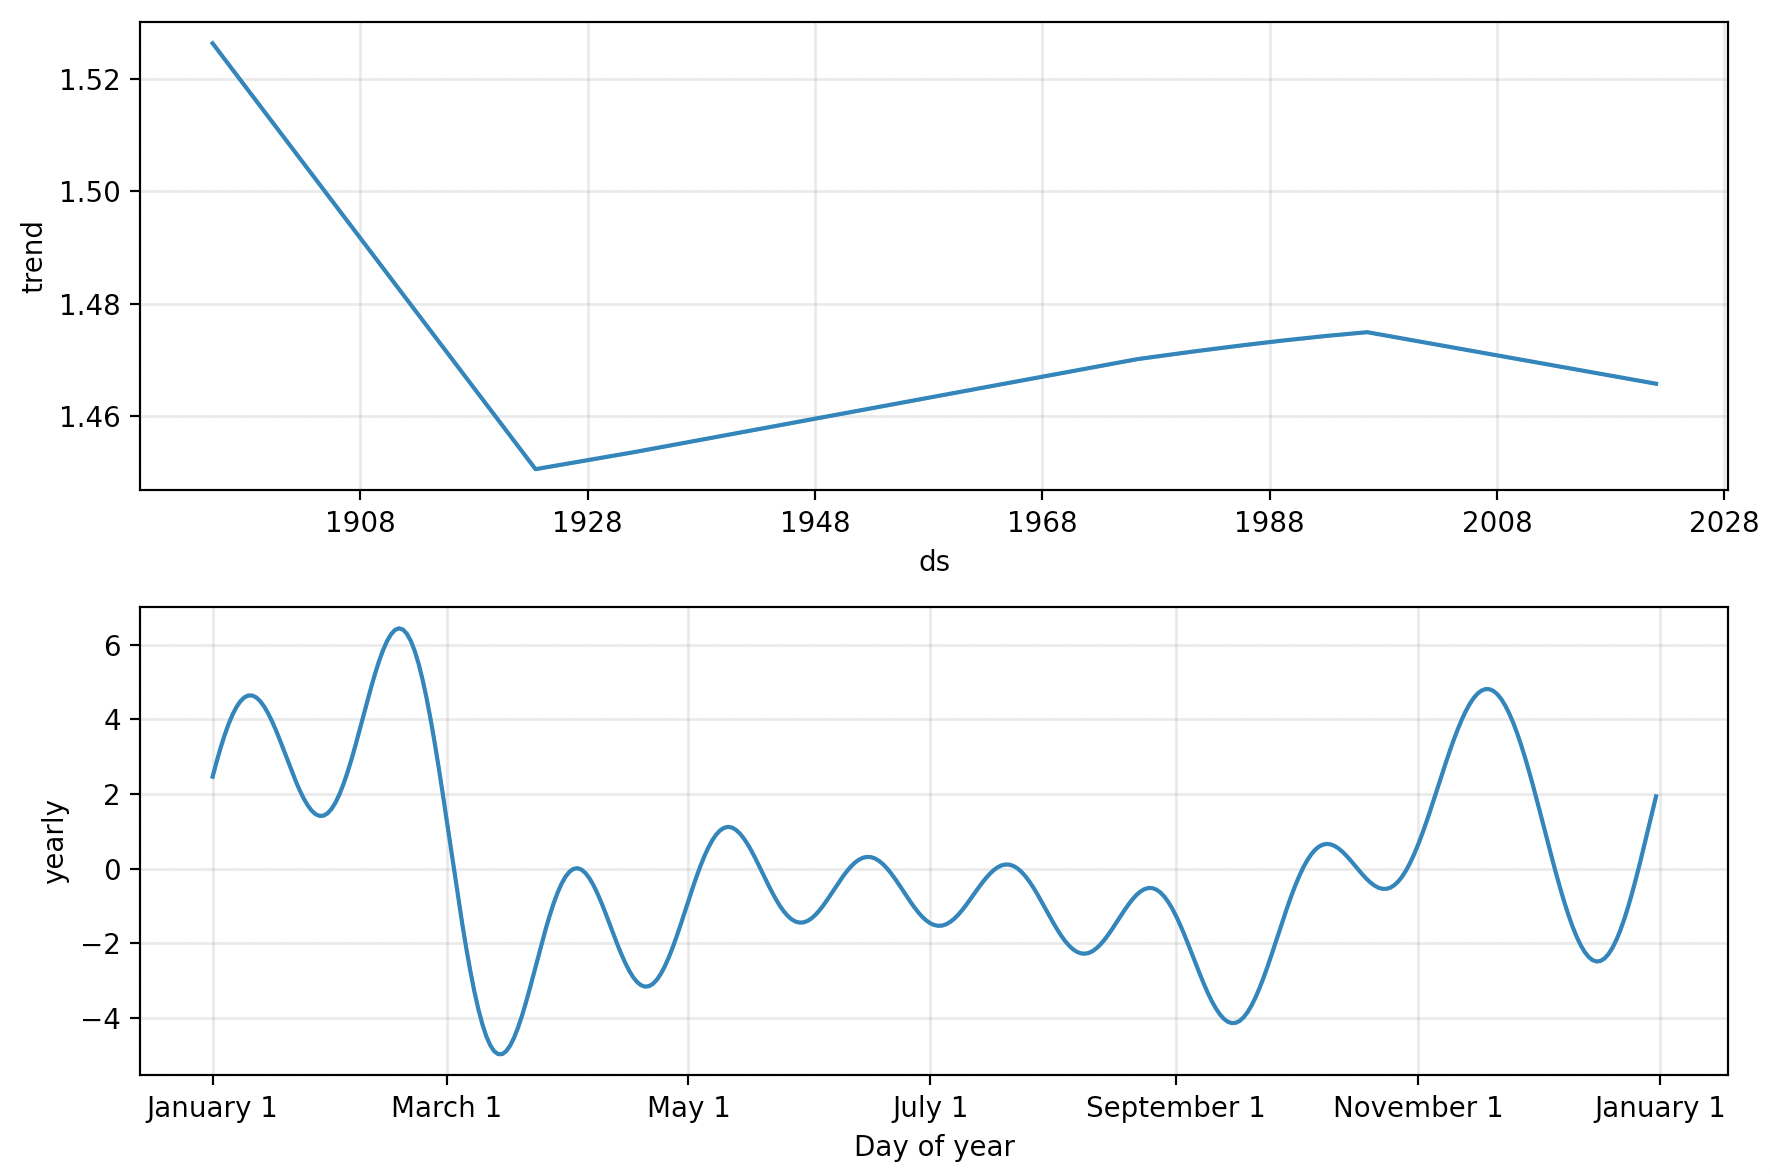
\includegraphics[width=10cm]{latex_template/AlamedaTrends.png}
    \caption{(Above) Overall trend of Alameda County precipitation; (Below) Yearly Seasonality Trend of Alameda County precipitation}
    \label{fig:galaxy}
\end{figure}


The graphs above were generated by Prophet after analyzing the historical data for Alameda County. A more detailed explanation of how Prophet works will be discussed in section 3, but the top chart shows the overall trend of the monthly precipitation data for this particular county, and the bottom chart shows the yearly seasonality pattern of the data. With this data, unlike the growth chart of a stock, there is no noticeable pattern with the overall trend. This makes forecasting values more difficult. However, there is still valuable information that Prophet is able to extract. The trend chart shows the minimum value of monthly precipitation at around 1928, which coincidentally was the start of one of California's worst droughts, as well as the Dust Bowl. 

The second chart demonstrates the seasonality of the data determined by Prophet. A seasonal pattern are changes in the data values that are regularly repeated over the same time period. In this case, there is a very logical pattern: there are higher monthly precipitation values in the fall and winter months, and lower in the summer months. An article published in The Startup on times series forecasts states that "a particular time series is thought to be composed of components called level, trend, seasonality, and noise \cite{seasonal}." A time series is considered to be some combination of these four components; however, trends and seasonality are optional and are not always present. When these are present, it is very important to account for that in the model, otherwise the natural dip in precipitation from March to May may confuse the model into thinking a drought is imminent. Prophet makes dealing with this especially simple. 


\section{Prophet and Forecasting Model}
Prophet is an open-source forecasting tool \cite{prophet} released by Facebook offering simple and completely automatic prediction ability. Its goal was to allow both experts and non-experts to make high quality forecasts. It produces fast, reliable, and accurate forecasts, but also accommodates experts in particular domains by the inclusion of many easily interpretable parameters that can be tweaked. Prophet is optimized for data that exhibits some sort of historical trend (particularly ones with a non-linear growth curve), has a good amount of either weekly or monthly observations, and displays either weekly or yearly seasonality. 

At its core, Prophet is an additive regression model, with four main components \cite{prophet}: 
\begin{itemize}
  \item A piecewise linear or logistic growth curve trend. Prophet automatically detects changes in trends by selecting changepoints from the data.
  \item A yearly seasonal component modeled using Fourier series.
  \item A weekly seasonal component using dummy variables.
  \item A user-provided list of important holidays.
\end{itemize}

Prophet attempts to solve the problems of complexity and accuracy with some of the other models commonly used for forecasting values. A few that I also considered using for this model are ARIMA, SARIMA, and Holt-Winters Exponential Smoothing. ARIMA stands for Auto-Regressive Integrated Moving Average models, which are among the most widely used time series forecasting techniques. These models combine two approaches: an autoregressive model where the forecasts correspond to a linear combination of past values, and a moving average model where the forecasts correspond to a linear combination of past forecast errors \cite{arima}. The main reasons that Prophet was chosen over this are that Prophet was much simpler to use and did not require as deep an understanding of the underlying math to use, and Prophet is more robust to missing data and shifts in the trend, and is especially good at handling outliers. 

The other method, Holt-Winters ES (Exponential Smoothing), was used in the original iteration of this model. This method is comprised of four forecasting techniques stacked one over the other: weighted averages, exponential smoothing, Holt exponential smoothing, and Holt-Winters exponential smoothing \cite{holts}. This model is similar to SARIMA in that it also accounts for the same seasonality trends, but instead uses exponential smoothing, which means that assigns a higher weight to more recent historical data compared to older data. Similar to Prophet, this method accounts for all four aspects of time series (level, trend, seasonality, noise); however, it was much more difficult to find the perfect values for these parameters. Prophet has automatic methods for tuning these, and was much simpler to configure for this model. 


\begin{figure}[htp]
    \centering
    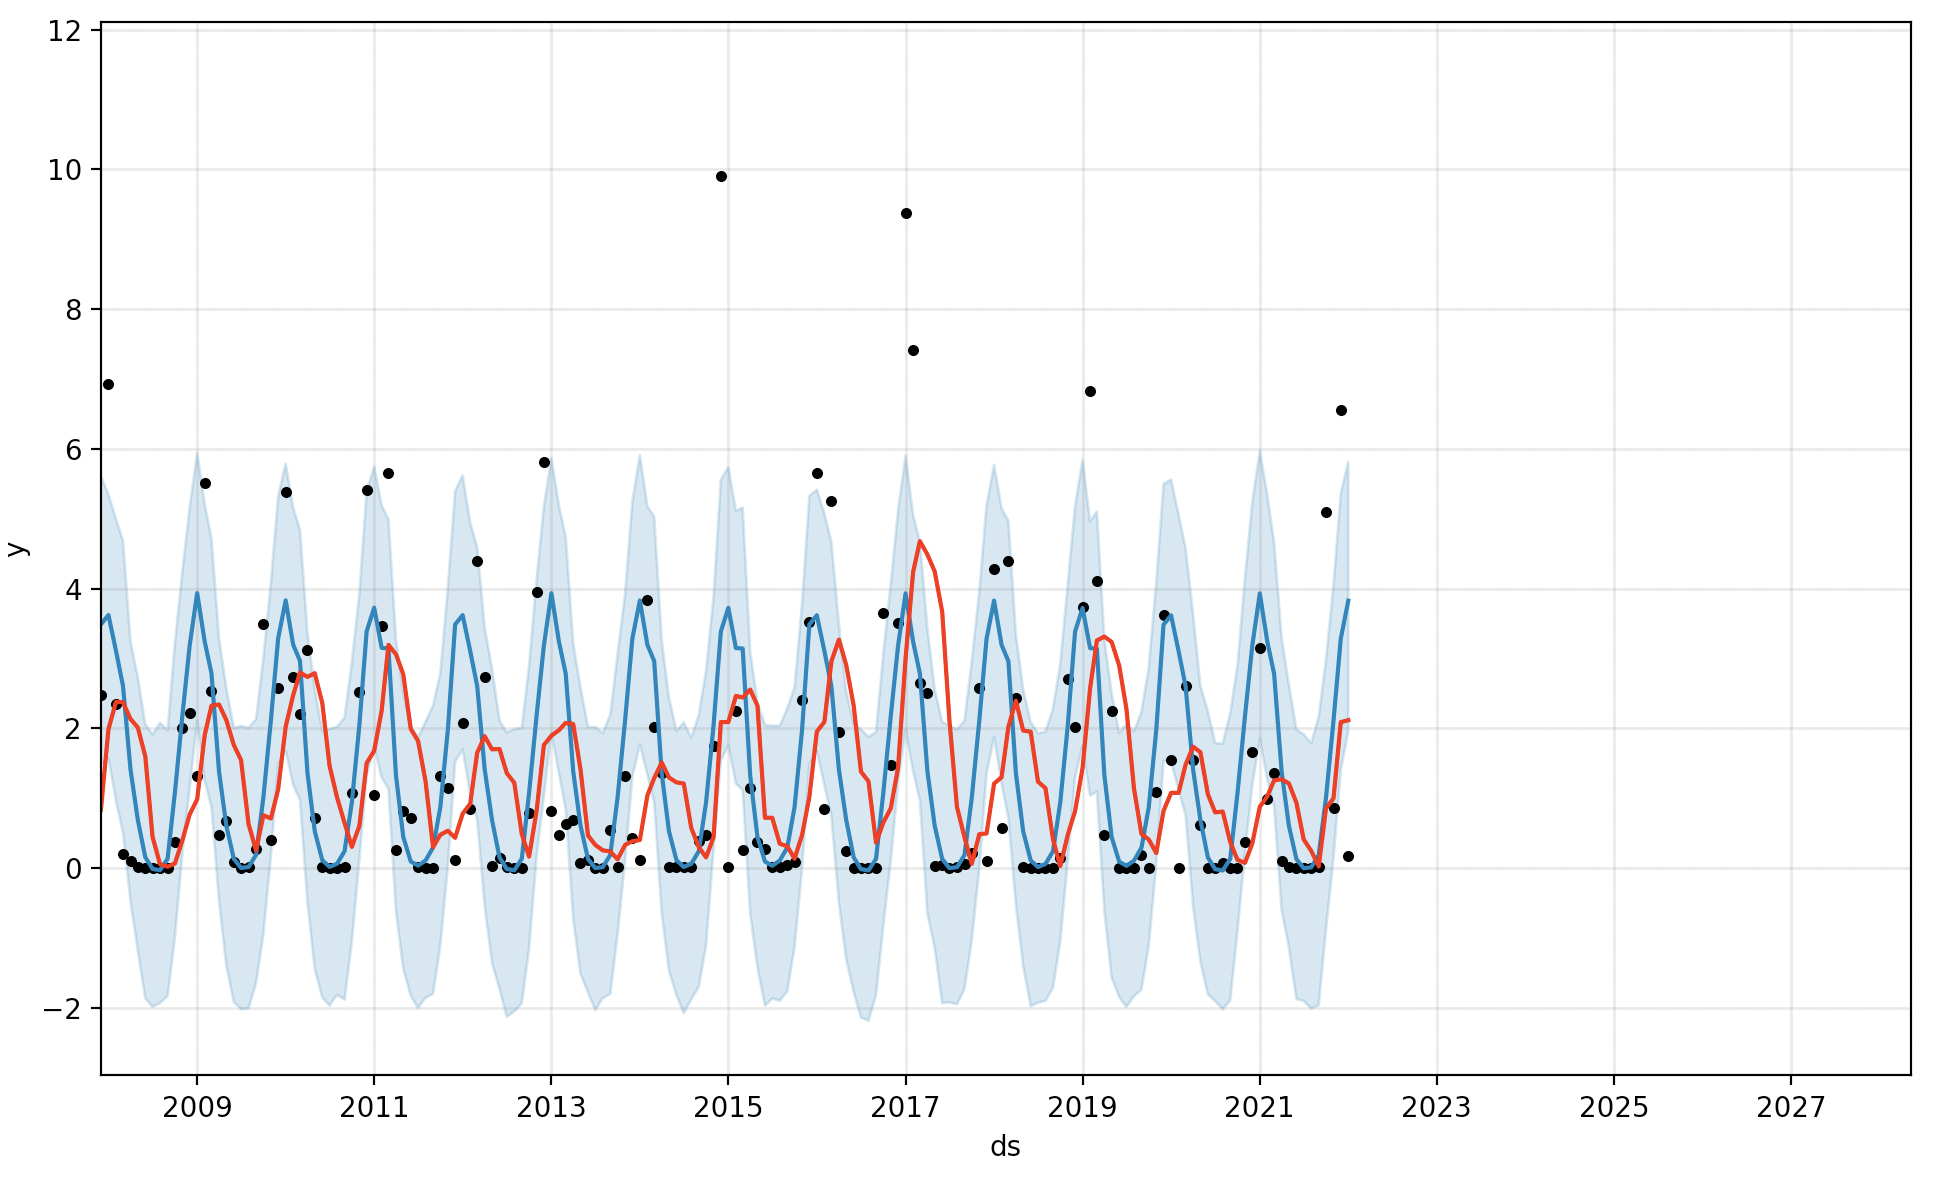
\includegraphics[width=10cm]{latex_template/PredictionWConfidenceBounds.png}
    \caption{Last years of Alameda County monthly precipitation data. The red line is a rolling mean with a 6-month window of the data. The dark blue line is the forecasting result generated by Prophet, along with the light blue shadings indicating confidence intervals}
    \label{fig:galaxy}
\end{figure}


The plot above was produced by Prophet. It shows the last decade from the data set for Alameda County's precipitation data. The dark blue line indicates the forecasted values using the optimal parameters. The light blue confidence intervals can be seen to extend below the minimum recorded values, as monthly precipitation in inches cannot be negative. An option to cap the minimum value was used. The idea of the model was to generate a number for each county based on the precipitation data that would represent its level of danger for having a drought. To accomplish this, the Prophet-forecasted values were used as 'expected' values. Over the last 6 months of recorded data for each county, the sum of the difference between these 'expected' values and the actual recorded value was calculated and treated as the danger level. Prophet does offer the ability to make forecasts as far into the future as needed; however, this seemed like the best solution for the following reasons. First, the farther out you predict, the less accurate the forecast is. As discussed in section 2, many of these underlying models rely on the trends and values close by, and this becomes weaker the further out you try to predict. Secondly, we are trying to predict droughts which would be an extreme deviation from normal data trends. Prophet or any other model will not produce predictions with a chance of being significantly off, and so we cannot base the danger factor for a county based off the prediction alone. Instead, the forecasted value was treated as what the expected rainfall should have been, and by comparing it to the actual values to see if the expected is being met, we get a far better indicator of drought. 


\section{Results and Conclusion}


\begin{figure}[htp]
    \centering
    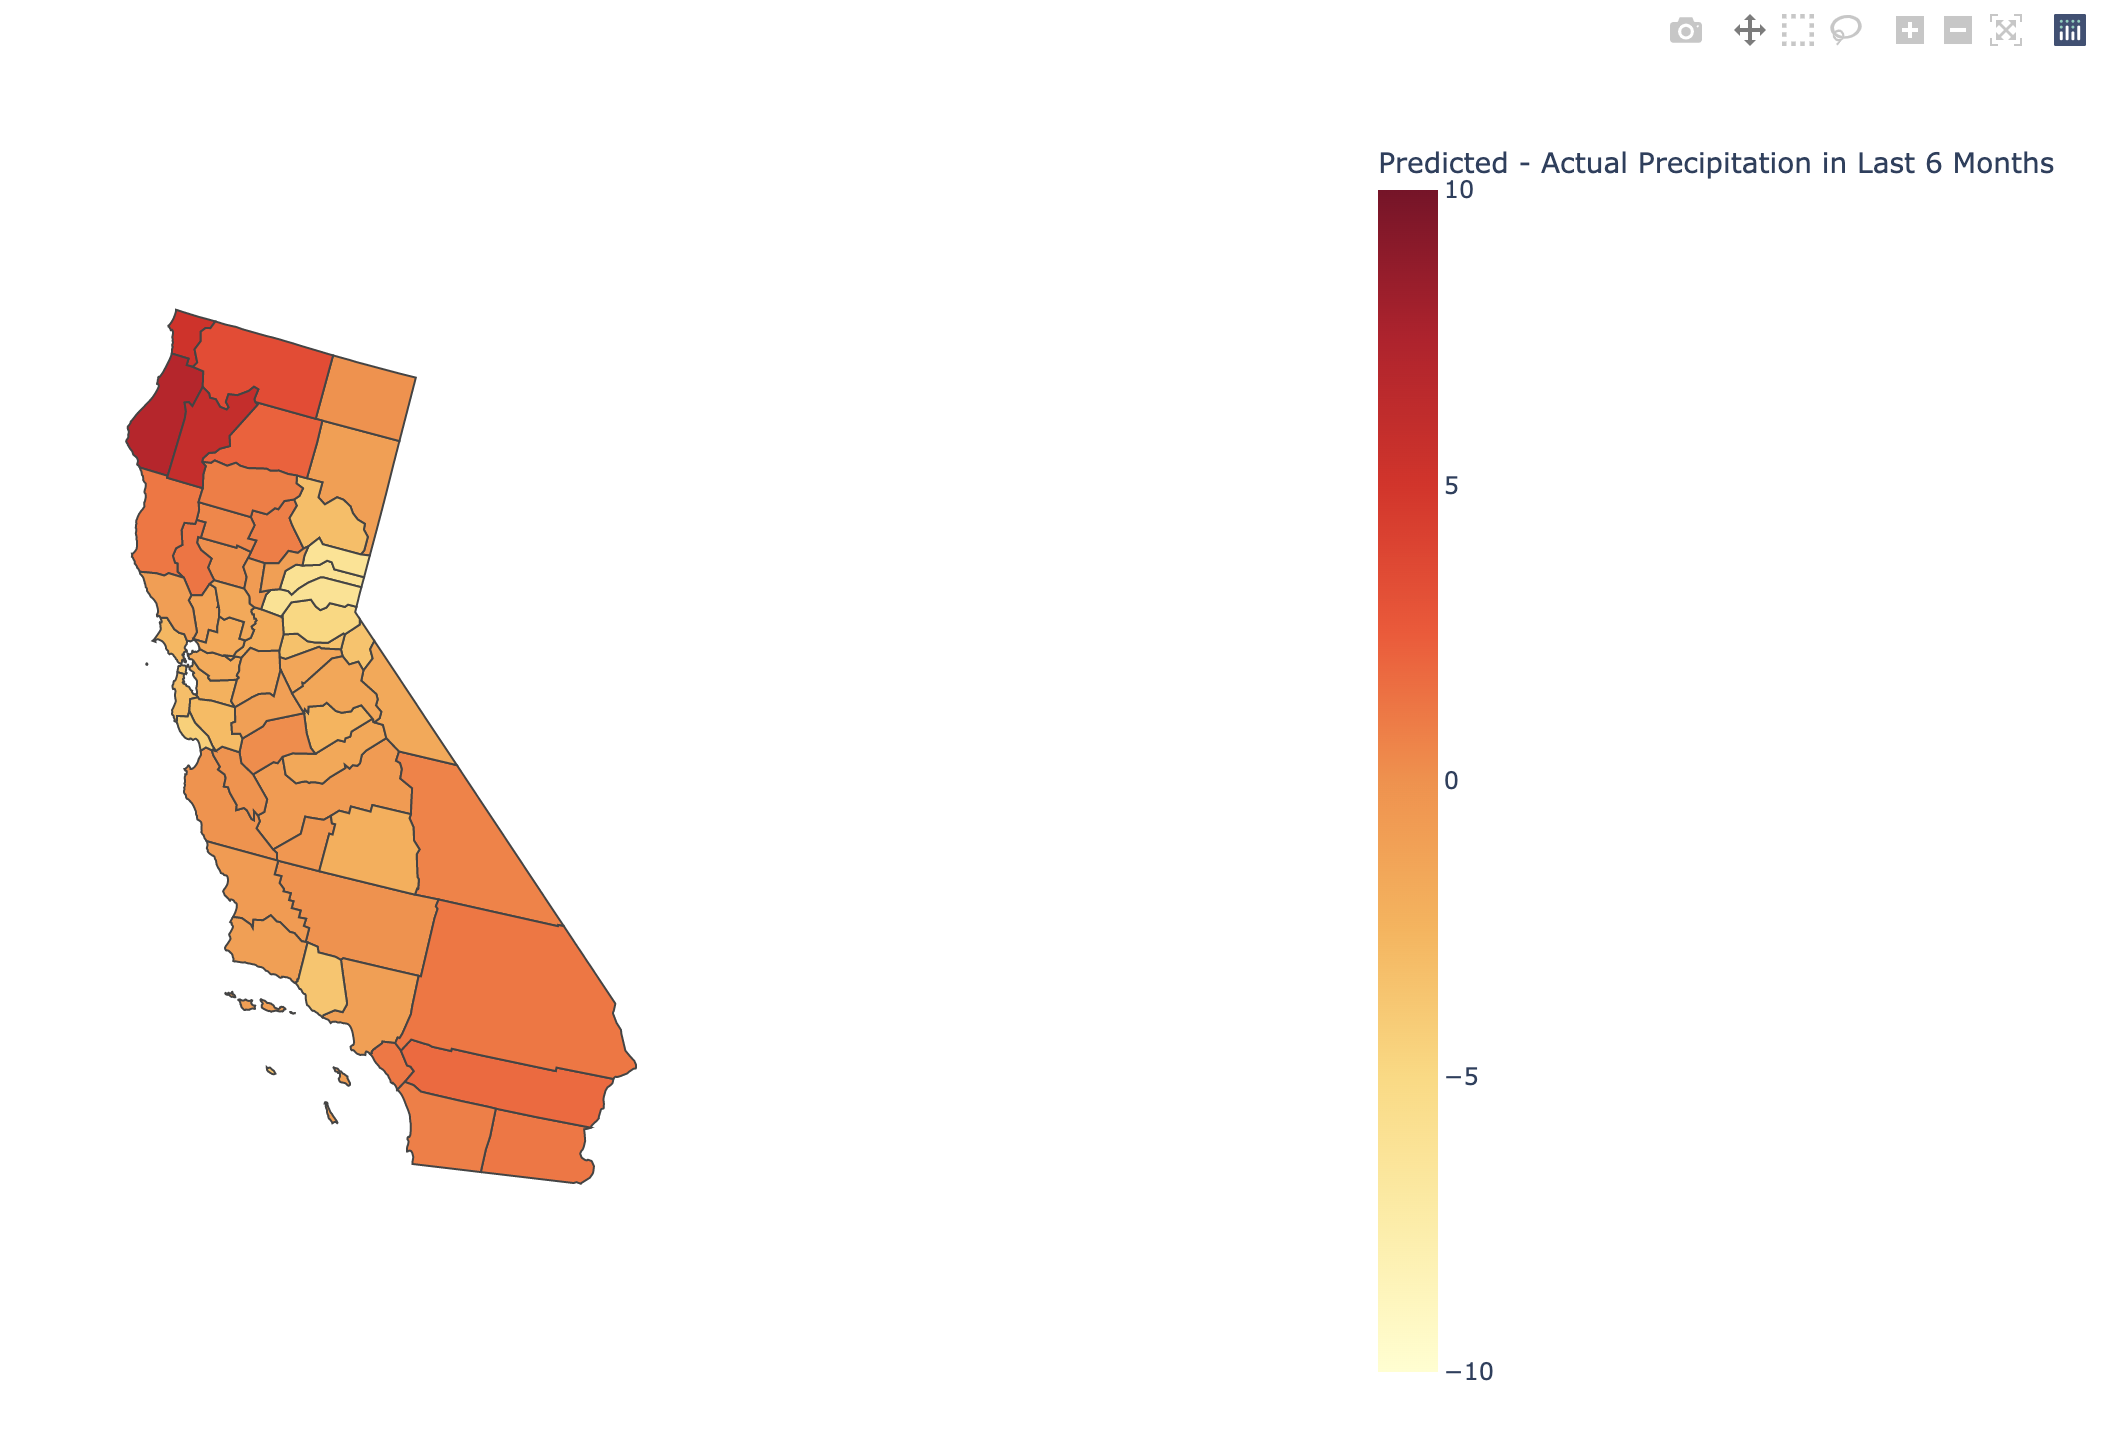
\includegraphics[width=10cm]{latex_template/FinalMap.png}
    \caption{Choropleth map indicating level of danger of drought per county}
    \label{fig:galaxy}
\end{figure}


Using Prophet, I constructed a model that accurately and quickly generated a value representing the danger level that a county was in of facing a drought. The final piece was to create a convenient way to deliver these results in a visual and easily-digestable manner. To do so, using the numbers generated by the model and stored in a dictionary linking the value to the county name it was assigned to. This was fed into another program that generated the choropleth map seen above, which is a map that uses shading to represent a quantity of some sort. As our value was the summation of the difference between the expected and actual rainfall, the more positive the value was the larger the risk of drought was. To demonstrate this, we used dark red to indicate the upper end of the spectrum, and light yellow to show the lowest risk counties. This satisfied the original goal of this model; to have an accurate model that can also display its results in a sleek, immediately understandable manner. 

My model determined that the northwestern region of California, specifically Humboldt County, is at highest risk of drought. This is corroborated by the drought prediction from the US Drought Monitor \cite{drought}, and this data was used to validate my results. I was not aiming to produce the exact same choropleth map as the US Drought Monitor, as my goal was to see if just precipitation alone could produce a good enough model to approximate this, and my goal was successful. Using multiple validation folds, I discovered that a 6-month period of comparison in my model was optimal for producing the most accurate results. I was also able to tune other hyperparameters in the Prophet forecasting using this. Through this I was able to say that my assumption made in section 2 about precipitation being the main indicator of drought was proven successful because the model created from just rainfall data produced a very good model. Furthermore, I also concluded that using time series forecasting models was successful as well, as both the original attempt using Holt-Winters and the final iteration using Prophet produced good results. The data and the problem set had all the right qualifications for needing this type of model, in that it had a non-linear overall trend and displayed seasonality. For this reasons, along with others explained in previous sections, Prophet was a great choice over other models, mostly for its combination of ease and convenience, and accuracy. 




\bibliographystyle{plain}
\bibliography{sample}

\end{document}
